% \documentclass[jou,apacite]{apa6}
\documentclass[doc,apacite,12pt]{apa6}

%-------------------------
 % Packages

\usepackage[normalem]{ulem}
\usepackage{listings}

\usepackage{url}

\usepackage{graphicx}
\graphicspath{ {resources/} }

%-------------------------
 % Commands
\newcommand{\bx}{BlaTeX }
\newcommand{\lx}{LaTeX } 
%Need space after to make sure the space is inserted after command

%-------------------------
 % The Title of your paper

\title{BlaTeX}
\shorttitle{R. Shah}

%-------------------------
 % Author

\author{Rushi Shah}
\affiliation{TJHSST}

%-------------------------
 % Abstract               
%-------------------------
\abstract{Write your blog in LaTeX.}

\begin{document}
\maketitle    

% final product
% design decisions
% internals of tech used
% steps taken to produce this (chronological)
         
%-------------------------
 % Introduction               
%-------------------------
\section{Introduction}
%Motivation for research.

Markdown and HTML are the standard tools used to write your every day tech blog with. But they have pretty weak support for embedding mathematical formulas, and are not conducive to writing for an extended period of time. Plus, they aren't even Turing complete! So instead of writing posts in Markdown, my project allows writers to create posts in LaTeX (a powerful markup language) and generate a static-site that can be deployed to any hosting service (like TJ's servers).

%-------------------------
 % Background 
%-------------------------
\section{Background}

Typically, static-sites like blogs are built with a tool called Jekyll. This Ruby project compiles Markdown posts into a static HTML site. \bx is similar, it is a static-site compiler written in Haskell that compiles LaTeX posts into a deploy-able site. The following description has been edited to highlight the minor differences between Jekyll and \bx:

\sout{Jekyll} BlaTeX is a simple, blog-aware, static site generator. It takes a template directory containing \sout{raw text files in various formats} LaTeX files\sout{, runs it through a converter (like Markdown) and our Liquid renderer,} and spits out a complete, ready-to-publish static website suitable for serving with your favorite web server. \sout{Jekyll also happens to be the engine behind GitHub Pages, which means} you can use \sout{Jekyll} BlaTeX to host your project's page, blog, or website from GitHub's servers for free.

Another popular content-management system for blogging is Wordpress. However, Wordpress posts are edited in the Wordpress Administration Panel as ``What you see is what you get''. Neither Markdown nor LaTeX are ``What you see is what you get'', and thus Wordpress caters to a completely different audience (a group of mostly non-technical authors). 

%-------------------------
 % Development
%-------------------------
\section{Development \& Techniques}

\subsubsection{Requirements}
% Technical requirements should be more about the requirements that would make this project a success
This command line utility requires the Haskell Platform and LaTeX. The Haskell Platform includes GHC (a Haskell compiler) and Cabal, which is Haskell's primary package manager. LaTeX is needed to build LaTeX posts into their resulting PDFs. After the Haskell Platform has been installed, installing BlaTeX is simple:

\begin{lstlisting}
> cabal install blatex
\end{lstlisting}

\subsubsection{Overview}
% Briefly outline the method used to develop the project
The project is a command line utility that is written in Haskell. 

\subsubsection{Limitations}
% Equipment, time, materials, etc.

One potential limitation of this project is that it only compiles links to PDF files. Because LaTeX can't generate HTML, the blog will only be a series of interlinked PDF files rather than a series of interlinked HTML files. This is not necessarily a limitation, but it may interrupt the status quo of typical blogs made of HTML pages. 

In order to parse the user's LaTeX files into an abstract syntax tree that can be consumed by Haskell, this project uses a Haskell package called \texttt{HaTeX}. This is a wonderful package (most of the time). The problem arises in a specific parsing instance. In LaTeX, a math environment is defined between two dollar-signs (\texttt{\$MATH GOES HERE\$}). In order to use dollar-signs as actual dollar-signs (like ``You owe me \$5''), you use an escape character before the symbol (\textbackslash). This is an exception to the math environment rule. However, HaTeX is not programmed to catch this exception gracefully. It matches pairs of dollar-signs and treats everything in between as math. If there are an odd number of dollar signs, or only one (even if they are escaped properly) HaTeX will just flat out fail to parse the entire file and thus BlaTeX will similarly ignore the post. 

Dates are formatted in \texttt{DD MONTH YEAR} which contributes to the minimalist, classy theme of PDF blog posts; this date format is also used in the internal implementation. However, this becomes an issue if multiple posts are authored on same day because they will not be displayed in the correct order. 

\subsection{Research Theory and Design Criteria}
% Clearly and Thoroughly present project methods, theory and algorithms
% Expand upon process in detail – (what you did), making sure to represent a sufficient level of difficulty and complexity

\subsection{Developmental Procedures}
% Explain the steps you took such that your project could be repeated by others (how you did it)


\subsection{Internal Testing and Analysis}
% How did you test and validate your code?
This tool was written in Haskell, a statically-typed, functional, compiled programming language. The compiled nature filtered out most insidious bugs in the code. Haskell development is also strongly integrated with using a Haskell REPL. Thus, each function was experimented with in the REPL after being written and before being pushed to production. 

\subsection{User Interface Testing and Analysis}
% Explain your user validation test
% Present the results of your user validation test
% I literally used it to maintain my own blog
In order to test this project, I used it to create and maintain \url{http://rshah.org/blog}. Through my own use I discovered multiple improvements that could be made to the user interface and experience, which I promptly implemented. 

I also posted my project in a Facebook group for functional programming and recieved an overwhelmingly positive response: 
\begin{figure}[ht]
	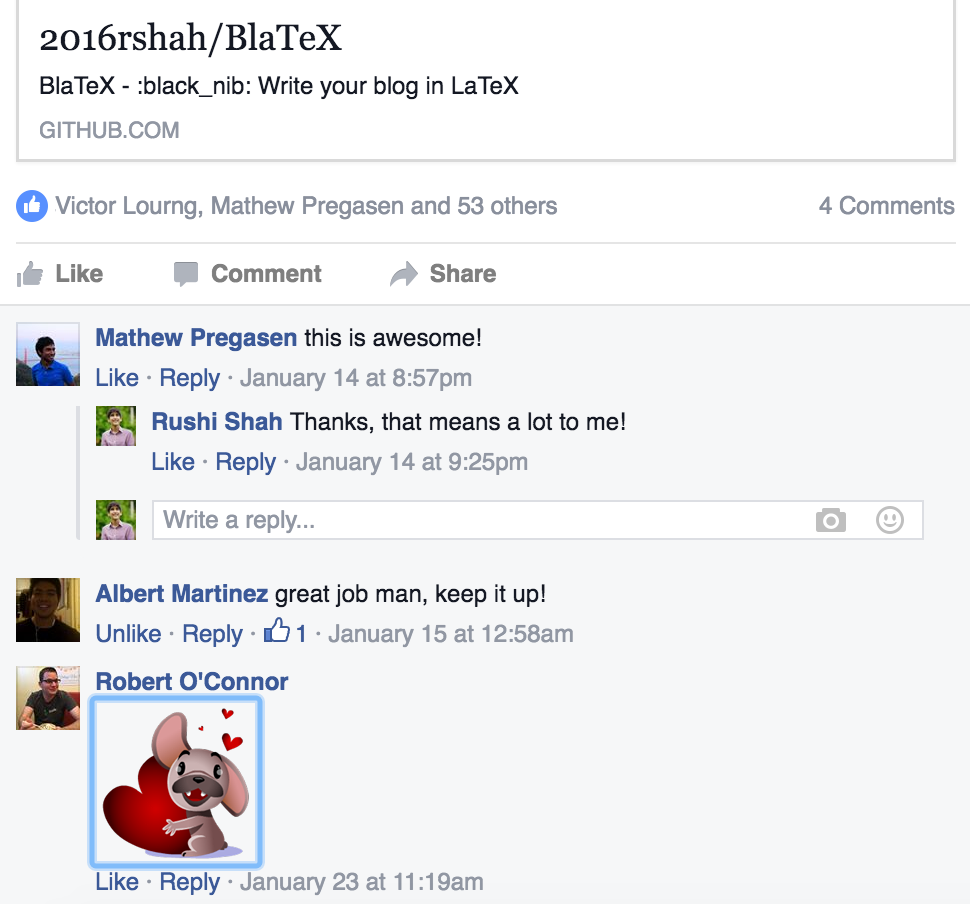
\includegraphics[width=\textwidth]{facebook}
	\centering
\end{figure}

It is also an open source project on Github, and met a similarly positive reaction from that community (with 17 Github ``stars''). 

\subsection{Visual representation of Results}
% Visually represent your project’s structure, results, algorithms

My blog at \url{http://rshah.org/blog} is a visual representation of a static site compiled with BlaTeX.

\begin{figure}[h]
	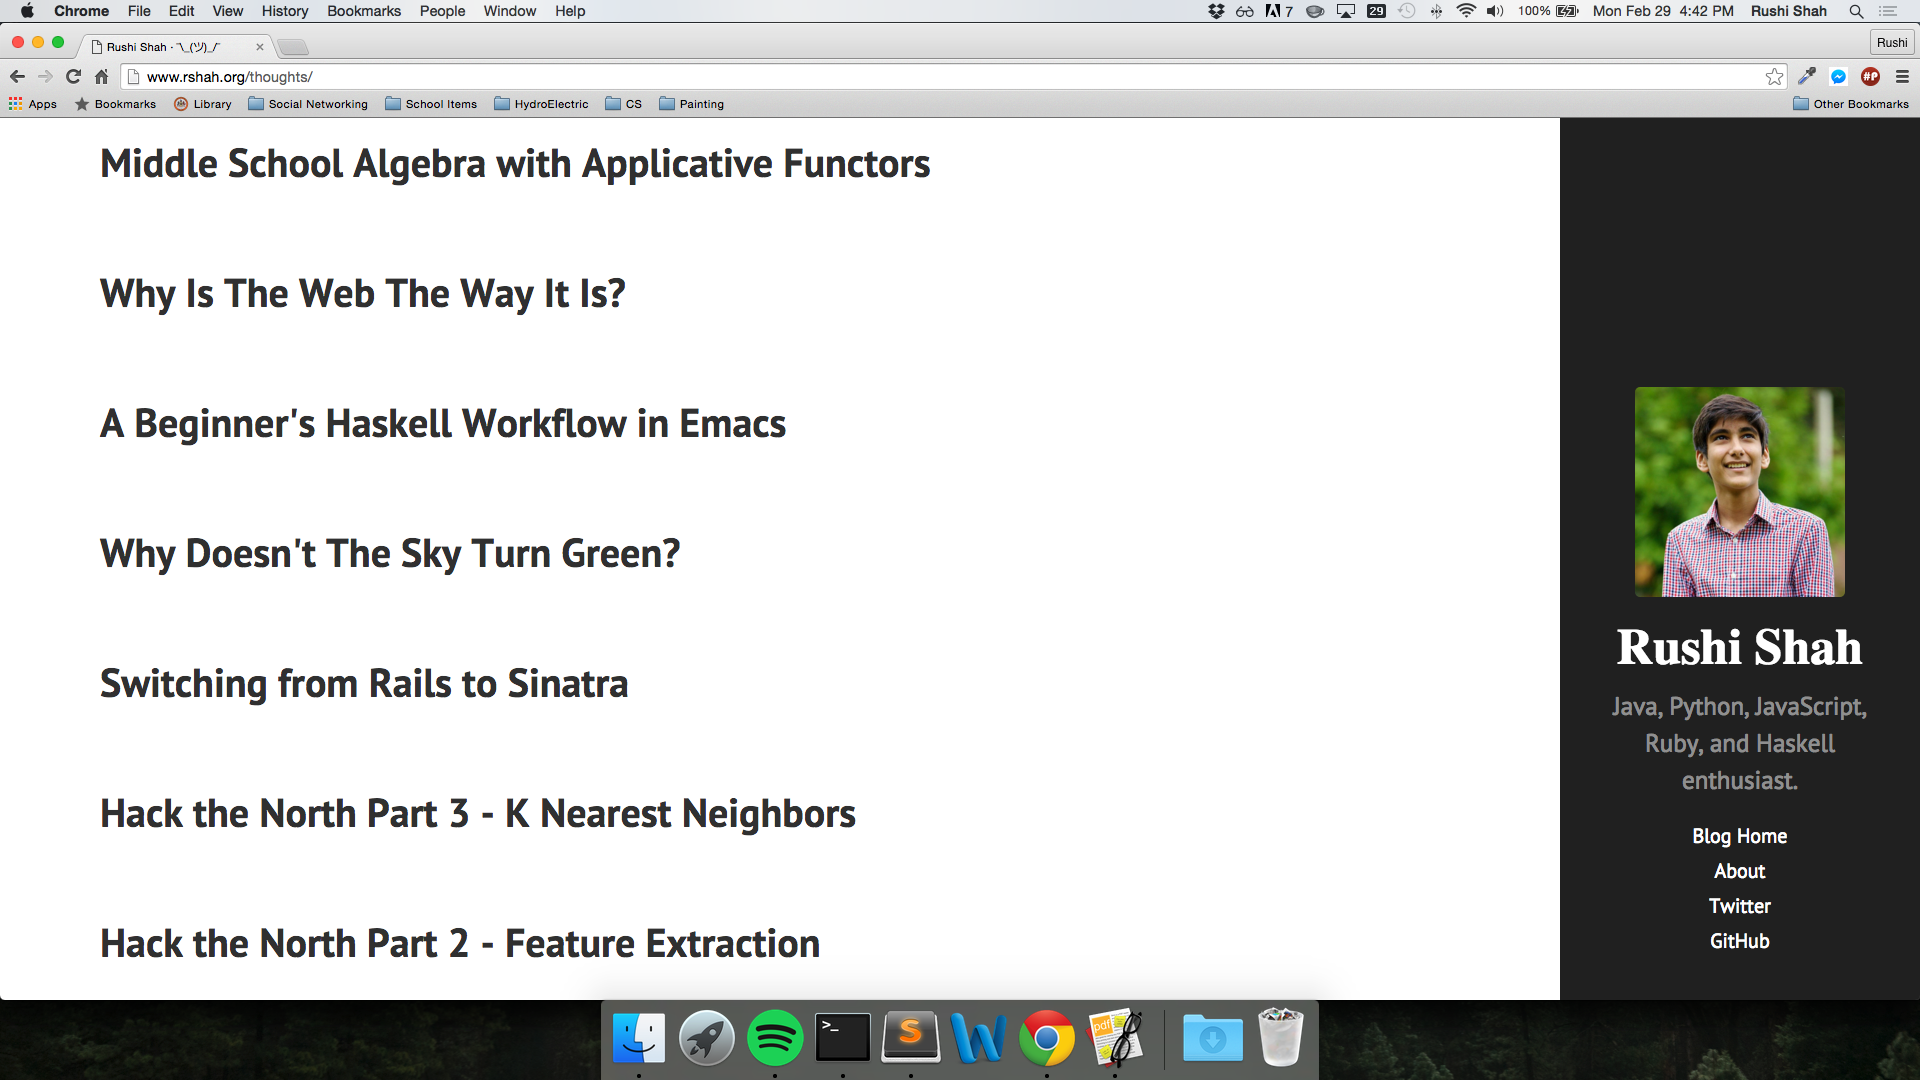
\includegraphics[width=\textwidth]{BlaTeX_screenshot}
	\centering
\end{figure}

%-------------------------
 % Results, Discussion, Conclusion              
%-------------------------
\section{Results, Discussion, and Conclusion}
% Presents the reader with the implication of the results.  
% Provide context so we can see what it all means.
% Provide specific, concise and thorough discussion of what you’ve learned.
% Specific recommendations of where the project can go from here

%-------------------------
 % Citations and References              
%-------------------------

% Citation of Einstein paper~\cite{Einstein}. Citation of Freud book~\cite{Freud}.

% \bibliography{final}

\end{document}
